\makeatletter
\def\input@path{{../styles/}{../../styles/}{../../../styles/}{../}{../../}{../../../}}
\makeatother
\documentclass{ee122_notes}
\input{macros.tex}
\input{preamble.tex}
\renewcommand{\releasedate}{April 8, 2026}


\begin{document}
\section*{EE 122/ME 141 Week 11, Lecture 2: Optimal control}
\subsection*{Instructor: \instructor}
\subsection*{Date: \releasedate}
\section{Announcements}
\begin{itemize}
    \item Problem set \#8 due on April 9, 2026 
    \item Problem set \#9 is out now and due on April 15, 2026
    \item Project milestone on completing the modeling due on April 12 (Sunday) at 11:59 PM.
\end{itemize}
\section{Learning Objective}
\begin{enumerate}
    \item Understand how to design a control law that optimizes the response of a closed-loop system.
    \item Apply the optimal control design to a simple example and compare the results to a state-feedback controller designed using pole placement.
\end{enumerate} 

\section{Review: Controller types}
In the class so far, we have studied the following controller designs:
\begin{enumerate}
    \item \textbf{PID control (Weeks 4 and 5)}: This is a frequency-domain technique using transfer functions and is the most widely used control design in practice.
    \item \textbf{Pole placement (Weeks 7-9)}: This control design technique could be in frequency-domain (by comparing the characteristic polynomial of the closed-loop system to a desired characteristic polynomial) or in time-domain (by comparing the state-space representation of the closed-loop system to a desired state-space representation using the controllable canonical form). 
    \item \textbf{State-feedback control (Week 9-10)}: This is a time-domain technique using state-space representations and uses all states to design the control law. To find the state-feedback gain, we can use pole placement or other approaches.
    \item \textbf{Integral-augmented state-feedback control (Week 11)}: In the previous lecture, we saw how to augment the state-space representation of a system with an integral state to design a controller that can achieve zero steady-state error.
    \item \textbf{Optimal control (Week 11: today)}: This is a time-domain technique using state-space representations and designs a control law that optimizes the response of the closed-loop system according to a specified cost function.
\end{enumerate}
\section{State-feedback control}
So far we have seen the following control design problem in the state-space representation. Given an open-loop system 
\begin{equation}
    \dot{x} = Ax + Bu, \qquad y = Cx,
    \label{eq:open_loop}
\end{equation}

our goal is to design a control law $u = -Kx$ such that the closed-loop system
\begin{equation}
    \dot{x} = (A - BK)x, \qquad y = Cx,
    \label{eq:closed_loop}
\end{equation}
has desirable properties. As an example, we show in Figure~\ref{fig:ol_vs_cl} the pole locations on the complex plane to demonstrate how the closed-loop system achieves better performance than the open-loop system. 
%draw figure in tikz with complex plan, Re, and Im axes, and poles for open-loop mark them at -1,4 and -1,-4, with red X marks and poles for closed-loop mark them at -2,2 and -2,-2 with blue X marks.
\begin{figure}[ht]
    \centering
    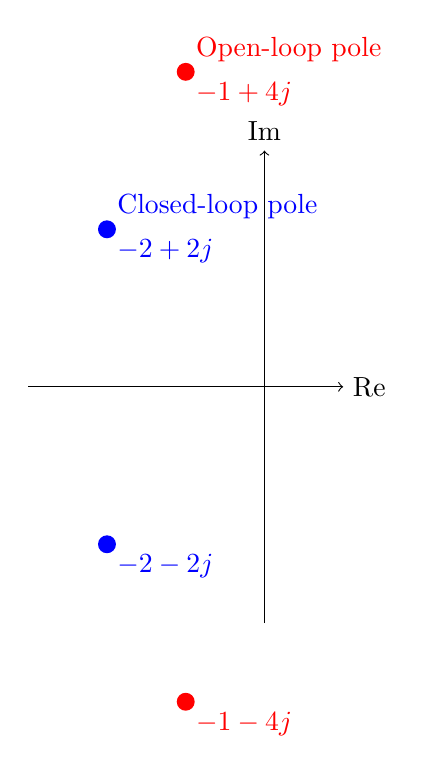
\begin{tikzpicture}
        % Draw axes
        \draw[->] (-3,0) -- (1,0) node[right] {Re};
        \draw[->] (0,-3) -- (0,3) node[above] {Im};

        % Draw open-loop poles
        \draw[red, thick] (-1,4) node[above right] {Open-loop pole} node[below right] {$-1 + 4j$} node[circle, draw, fill=red, inner sep=2pt] {};
        \draw[red, thick] (-1,-4) node[below right] {$-1 - 4j$} node[circle, draw, fill=red, inner sep=2pt] {};

        % Draw closed-loop poles
        \draw[blue, thick] (-2,2) node[above right] {Closed-loop pole} node[below right] {$-2 + 2j$} node[circle, draw, fill=blue, inner sep=2pt] {};
        \draw[blue, thick] (-2,-2) node[below right] {$-2 - 2j$} node[circle, draw, fill=blue, inner sep=2pt] {};
    \end{tikzpicture}
    \caption{Pole locations for open-loop and closed-loop systems.}
    \label{fig:ol_vs_cl}
\end{figure}

Now, see if you can answer the question below about the system given the pole locations in Figure~\ref{fig:ol_vs_cl}.
\begin{popquiz}
What does the closed-loop system achieve compared to the open-loop system? Try to name at least three properties of the closed-loop system that are better than the open-loop system based on the pole locations.
\popqsplit
\begin{itemize}
\item Faster response: The closed-loop poles are farther to the left in the complex plane compared to the open-loop poles, which indicates that the closed-loop system has a faster response than the open-loop system. Remember that the real part of the poles appear in the exponent of the system response: $e^{\text{Re}(p)t}$, where $p$ is a pole. Therefore, the more negative the real part of the pole, the faster the system response decays to zero.
\item Less oscillation: The closed-loop poles are closer to the real axis compared to the open-loop poles, which indicates that the closed-loop system has less oscillation / ``ringy'' response than the open-loop system. Remember that the imaginary part of the poles appear in the sinusoidal term of the system response: $\sin(\text{Im}(p)t)$, where $p$ is a pole. 
\item Convergence to the origin: Both the open-loop and closed-loop poles are in the left half of the complex plane, which indicates that both systems are stable and will converge to the origin. So, in this case, the closed-loop system performs same as the open-loop system in terms of stability and convergence to the origin. 
\end{itemize} 
\end{popquiz}
        
\section{Motivation for optimal control}
Building from the popquiz above, here are the properties that we usually want out of a closed-loop system:
\begin{itemize}
    \item The trajectories of the system must converge to the equilibrium point. (quick practical example: if you set your AC temperature to 70 degrees, you want the temperature to converge to that point, not stay where it was or diverge.)
    \item The trajectories of the system must converge to the equilibrium point fast. (quick practical example: you want the temperature in your room to reach 70 degrees quickly, not take forever to get there.)
    \item The trajectories of the system must not be too oscillatory. (quick practical example: you don't want the temperature in your room to oscillate between 68 and 72 degrees and eventually reach 70 degrees, you want it to smoothly converge to 70 degrees.)
\end{itemize}
The first two items above correspond to the state variables $x(t)$ and its clear that we want the absolute values of the state variables to be small at all times, which means we want to minimize \textit{something} that has the term $\| x(t) \|^2$. The last item above corresponds to the control input $u(t)$ --- since when the system oscillates more, it causes the control input to change more rapidly leading to excessive use of energy. Therefore, we also want to minimize \textit{something} that has the term $\| u(t) \|^2$. This motivates us to design a control law that minimizes a cost function of the form.
\section{LQR control}
Formally setting up the optimal control problem, we want to design a control law $u(t) = -Kx(t)$ that minimizes the cost function
\begin{equation}
    J = \int_0^{t_f} \left( x(t)^\top Q x(t) + u(t)^\top R u(t) \right) dt + x(t_f)^\top Q_f x(t_f),
    \label{eq:lqr_cost}
\end{equation}
where $Q$ is a positive semi-definite matrix of size $n \times n$, $R$ is a positive definite matrix of size $p \times p$ (if the control input is $p$-dimensional), and $Q_f$ is a positive semi-definite matrix of size $n \times n$. The first term in the cost function penalizes the state variables, the second term penalizes the control input, and the third term penalizes the final state at time $t_f$. The optimal control problem is to find the control law $u(t)$ that minimizes the cost function $J$ subject to the system dynamics given by $\dot{x} = Ax + Bu$.

This is called the Linear Quadratic Regulator (LQR) problem (notice the correspondence between the name and our choice of notation for the matrices: $Q$ and $R$). 

The LQR problem is simpler to solve when we assume that the time horizon is infinite (that is, $t_f = \infty$) and
all matrices are constants. Then, $P$ is constant and a solution to the continuous-time algebraic Riccati equation (CARE) given by
\begin{equation}
A^\top P + PA - PB R^{-1} B^\top P + Q = 0
\end{equation}
% AT S + SA − SBQ−1u B T S + Qx = 0. (7.33)
and the control law is given by 
\begin{equation}
    u(t) = -Kx(t) = -R^{-1} B^\top P x(t).
\end{equation}

\section{Example: LQR vs. pole placement}
We can solve the LQR problem in MATLAB or Python using the \texttt{lqr} function. It takes in the system matrices $A$ and $B$, and the cost matrices $Q$ and $R$, and returns the optimal state-feedback gain matrix $K$. 

\section{Next steps}
Make sure to read Section 7.5 in the textbook for more details on optimal control and the LQR problem. 

\end{document}